\subsubsection{Visualizar Menú}
En la figura \ref{fig:Diagrama de Secuencia - Visualizar Menú} mostramos el diagrama de secuencia correspondiente a la función de visualizar menú, aquí el usuario (empleado o administrador) puede elegir dos opciones:
\begin{itemize}
	\item \textbf{Gestión de Agenda:} Al elegir esta opción, el usuario podrá entrar a otra parte del sistema para que pueda interactuar con la base de datos mediante una interfaz gráfica. Es decir, que llevará a cabo las diversas tareas para poder tener un control sobre la información a cerca de los vehículos a reparar.
	\item \textbf{Gestión de Refacciones:} Si el usuario elige esta opción, el usuario podrá visualizar las refacciones que existen en el almacén del taller. En caso de que no exista la pieza que el necesita, podrá generar una solicitud dentro del mismo sistema. 
\end{itemize}
\begin{figure}[!h]
	\centering
	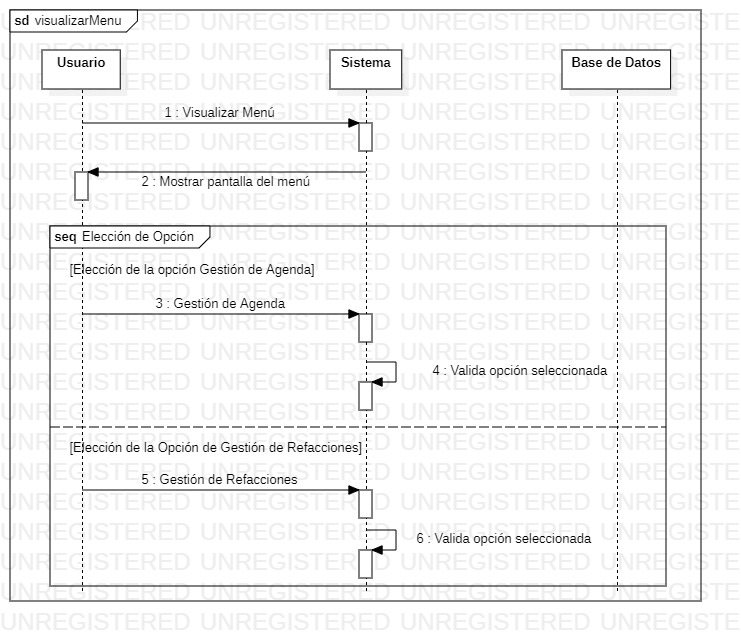
\includegraphics[width=0.9\textwidth]{./diseno/vprocesos/imagenes/visualizarMenu}
	\caption{Diagrama de Secuencia - Visualizar Menú}
	\label{fig:Diagrama de Secuencia - Visualizar Menú}
\end{figure}